%% LaTeX-Beamer template for KIT design
%% by Erik Burger, Christian Hammer
%% title picture by Klaus Krogmann
%%
%% version 2.4
%%
%% mostly compatible to KIT corporate design v2.0
%% http://intranet.kit.edu/gestaltungsrichtlinien.php
%%
%% Problems, bugs and comments to
%% burger@kit.edu

%% Class options
%%   aspect ratio options: 
%%   -- 16:9 (default)
%%   -- 4:3
%%   language options: 
%%   -- en (default)
%%   -- de
%%   position of navigation bar:
%%   -- navbarinline (default): bottom of the white canvas
%%   -- navbarinfooter : more compressed variant inside the footer
%%   -- navbarside : side bar at the left of the white canvas
%%   -- navbaroff : none
%% example: \documentclass[16:9,de,navbarinfooter]{sdqbeamer}
\documentclass[16:9,en,navbarinfooter]{sdqbeamer}

%% \documentclass{sdqbeamer} 

%% TITLE PICTURE

% if a custom picture is to be used on the title page, copy it into the 'logos'
% directory, in the line below, replace 'myimage' with the 
% filename (without extension) and uncomment the following line
% (picture proportions: 63 : 20 for standard, 169 : 40 for wide
% *.eps format if you use latex+dvips+ps2pdf, 
% *.jpg/*.png/*.pdf if you use pdflatex)

% \titleimage{myimage}

%% GROUP LOGO 

% for a custom group logo, copy your file into the 'logos'
% directory, insert the filename in the line below and uncomment it

\grouplogo{irlalr}

% (*.eps format if you use latex+dvips+ps2pdf,
% *.jpg/*.png/*.pdf if you use pdflatex)

%% GROUP NAME

% for groups other than SDQ, please insert in the line below and uncomment it
% \groupname{My group}

% the presentation starts here 

\author{Caspar Friedrich Maximilian Nagy}

%% Title (and possibly subtitle) of the thesis
\title{Solving Real-World Robot Manipulation Tasks with Deep Reinforcement Learning}
\subtitle{Box Pushing with Motion Primitives on a real Panda Robot}

% Bibliography 
\usepackage{dsfont}
%\usepackage{multimedia}
%\usepackage{media9}
\usepackage{booktabs}
\usepackage{longtable}
\usepackage{array}
\usepackage{algorithm}
\usepackage{algpseudocode}
\usepackage{pgfplots}
% \pgfplotsset{compat=1.15}
 \usepgfplotslibrary{groupplots}
\usepackage{subcaption}
\usepackage{pdflscape}
\usepackage{diagbox}
\usepackage{multicol}
\DeclareUnicodeCharacter{2212}{−}
\usepgfplotslibrary{groupplots,dateplot}
\usetikzlibrary{patterns,shapes.arrows}
\pgfplotsset{compat=newest}
\usepackage[citestyle=authoryear,bibstyle=numeric,hyperref,backend=biber%,style=verbose
]{biblatex}
\addbibresource{presentation.bib}
\bibhang1em
\usepackage{listings}
\begin{document}

%title page
\KITtitleframe{}

%table of contents


\begin{frame}
\frametitle{Agenda}
    \vspace{1cm}
\tableofcontents
\end{frame}

\section{Motion Primitive-Based (Re-)Planning Policy (MP3)}
\begin{frame}{Motion Primitive-Based (Re-)Planning Policy (MP3)}

\center 
    \vspace{1cm}
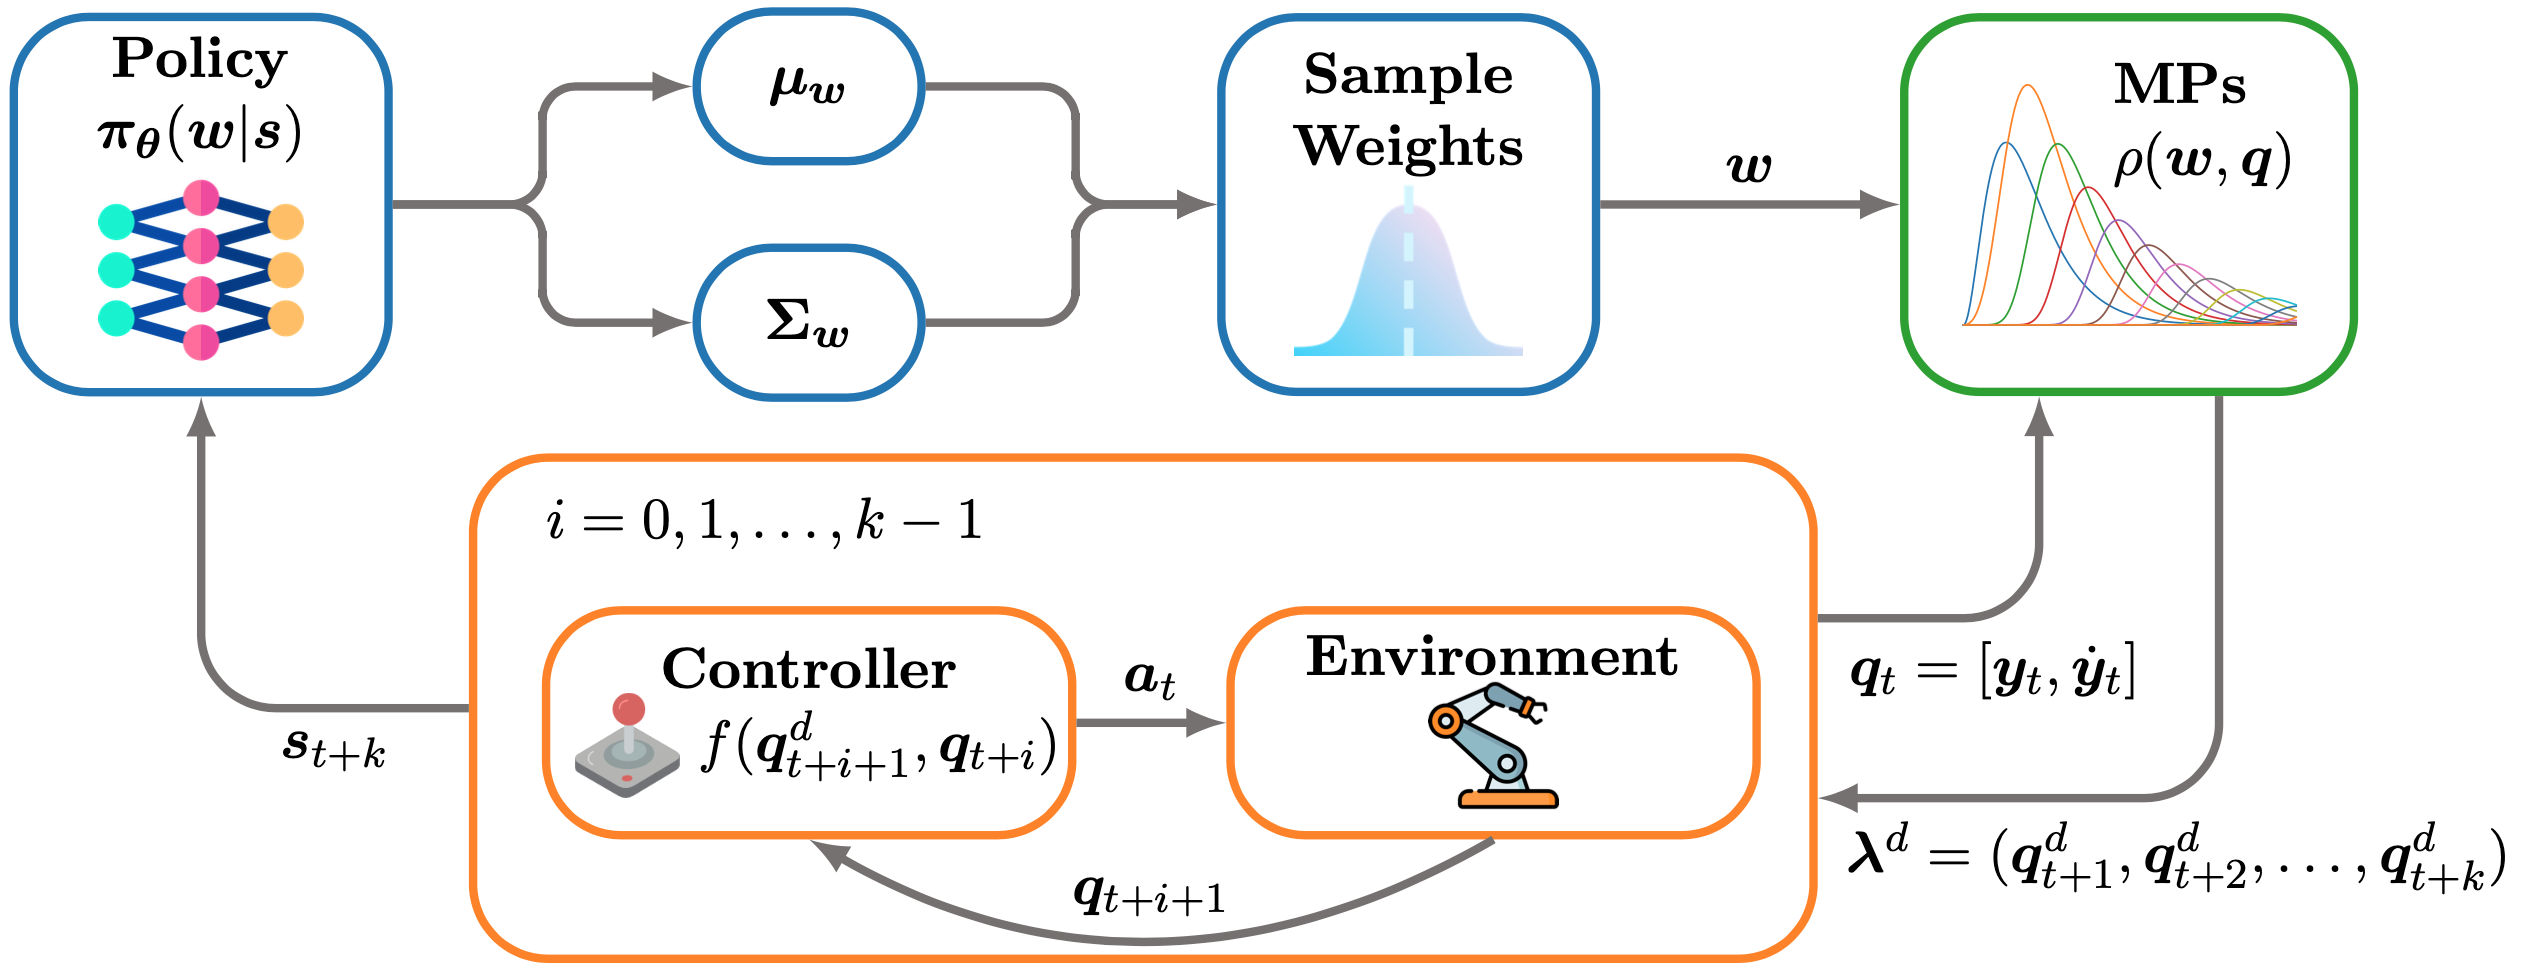
\includegraphics[width=.7\linewidth]{media/mp3.png}
\begin{itemize}
\item Blackbox and replanning variant
\item Works with sparse, non-markovian rewards
\item Generates smooth trajectories
\item Trained on-policy using Trust Region Projection Layers (TRPL)
\end{itemize}
\end{frame}

\subsection{MP3 in the Real World}
\begin{frame}{MP3 in the Real World}

\center 
    \vspace{1cm}
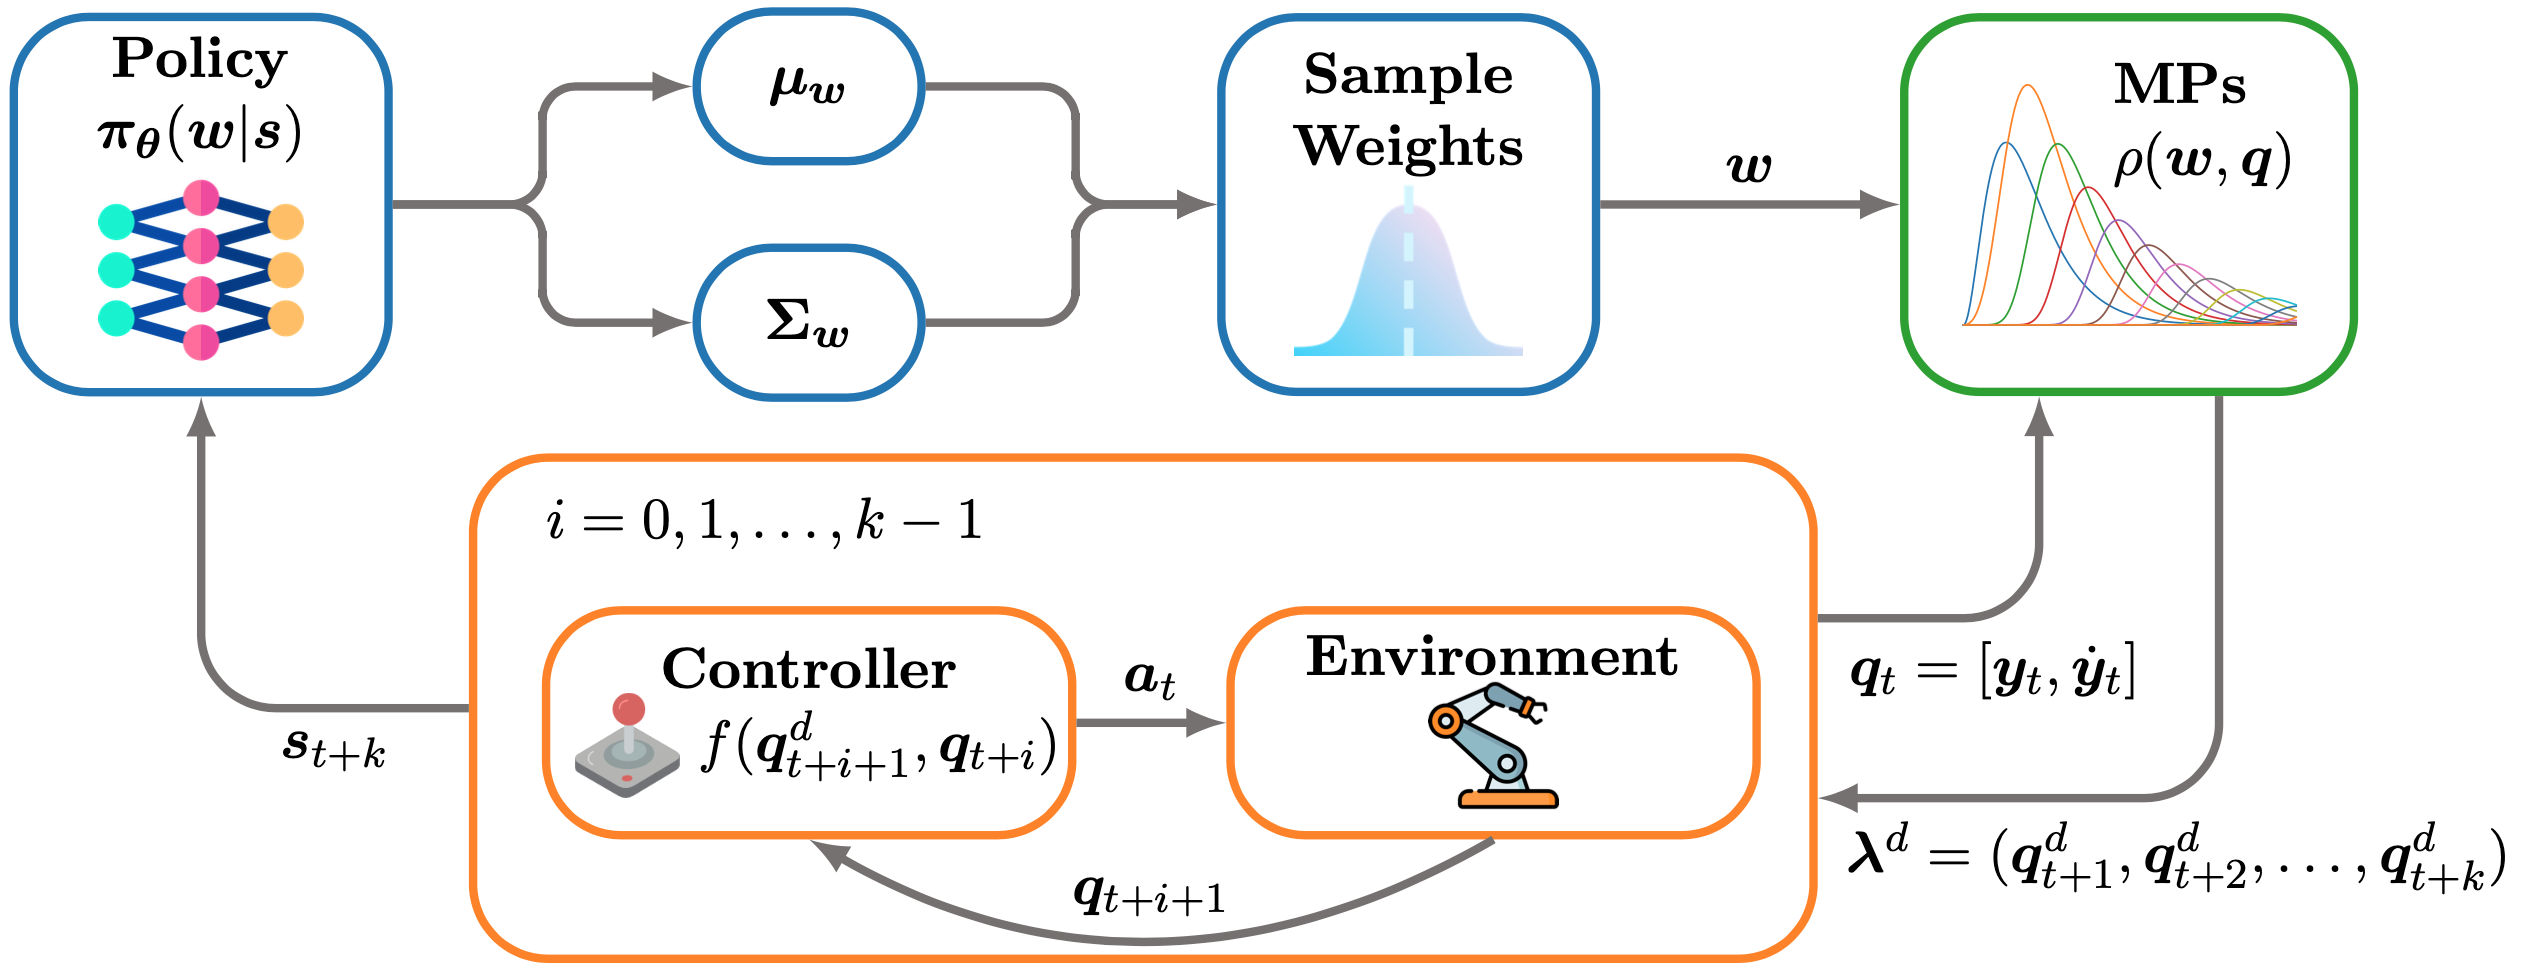
\includegraphics[width=.7\linewidth]{media/mp3.png}
   \begin{itemize}
           \item Contextual MPRL was never used on a real robot\dots will it work?
           \item How big is the sim2real gap?
           \item Do we need replanning?
           \item Is it better than step-based methods?
\end{itemize}
\end{frame}

\begin{frame}{Box Pushing}
\section{Box Pushing}

\begin{columns}[t]
    \begin{column}{0.5\textwidth}
        \begin{itemize}
            \item Goal: Use a ``finger'' to push a box to a target pose
                \begin{itemize}
                    \item Random start pose
                    \item Fixed target pose
                \end{itemize}
        \end{itemize}
    \end{column}
    \begin{column}{0.5\textwidth}
        \begin{itemize}
                \item Challenges
                    \begin{itemize}
                            \item Underactuated system
                            \item Complex table-box interactions
                            \item Complex Panda kinematic 
                            \item Trajectories must be safe and executable
                    \end{itemize}
        \end{itemize}
    \end{column}


\end{columns}
\center
    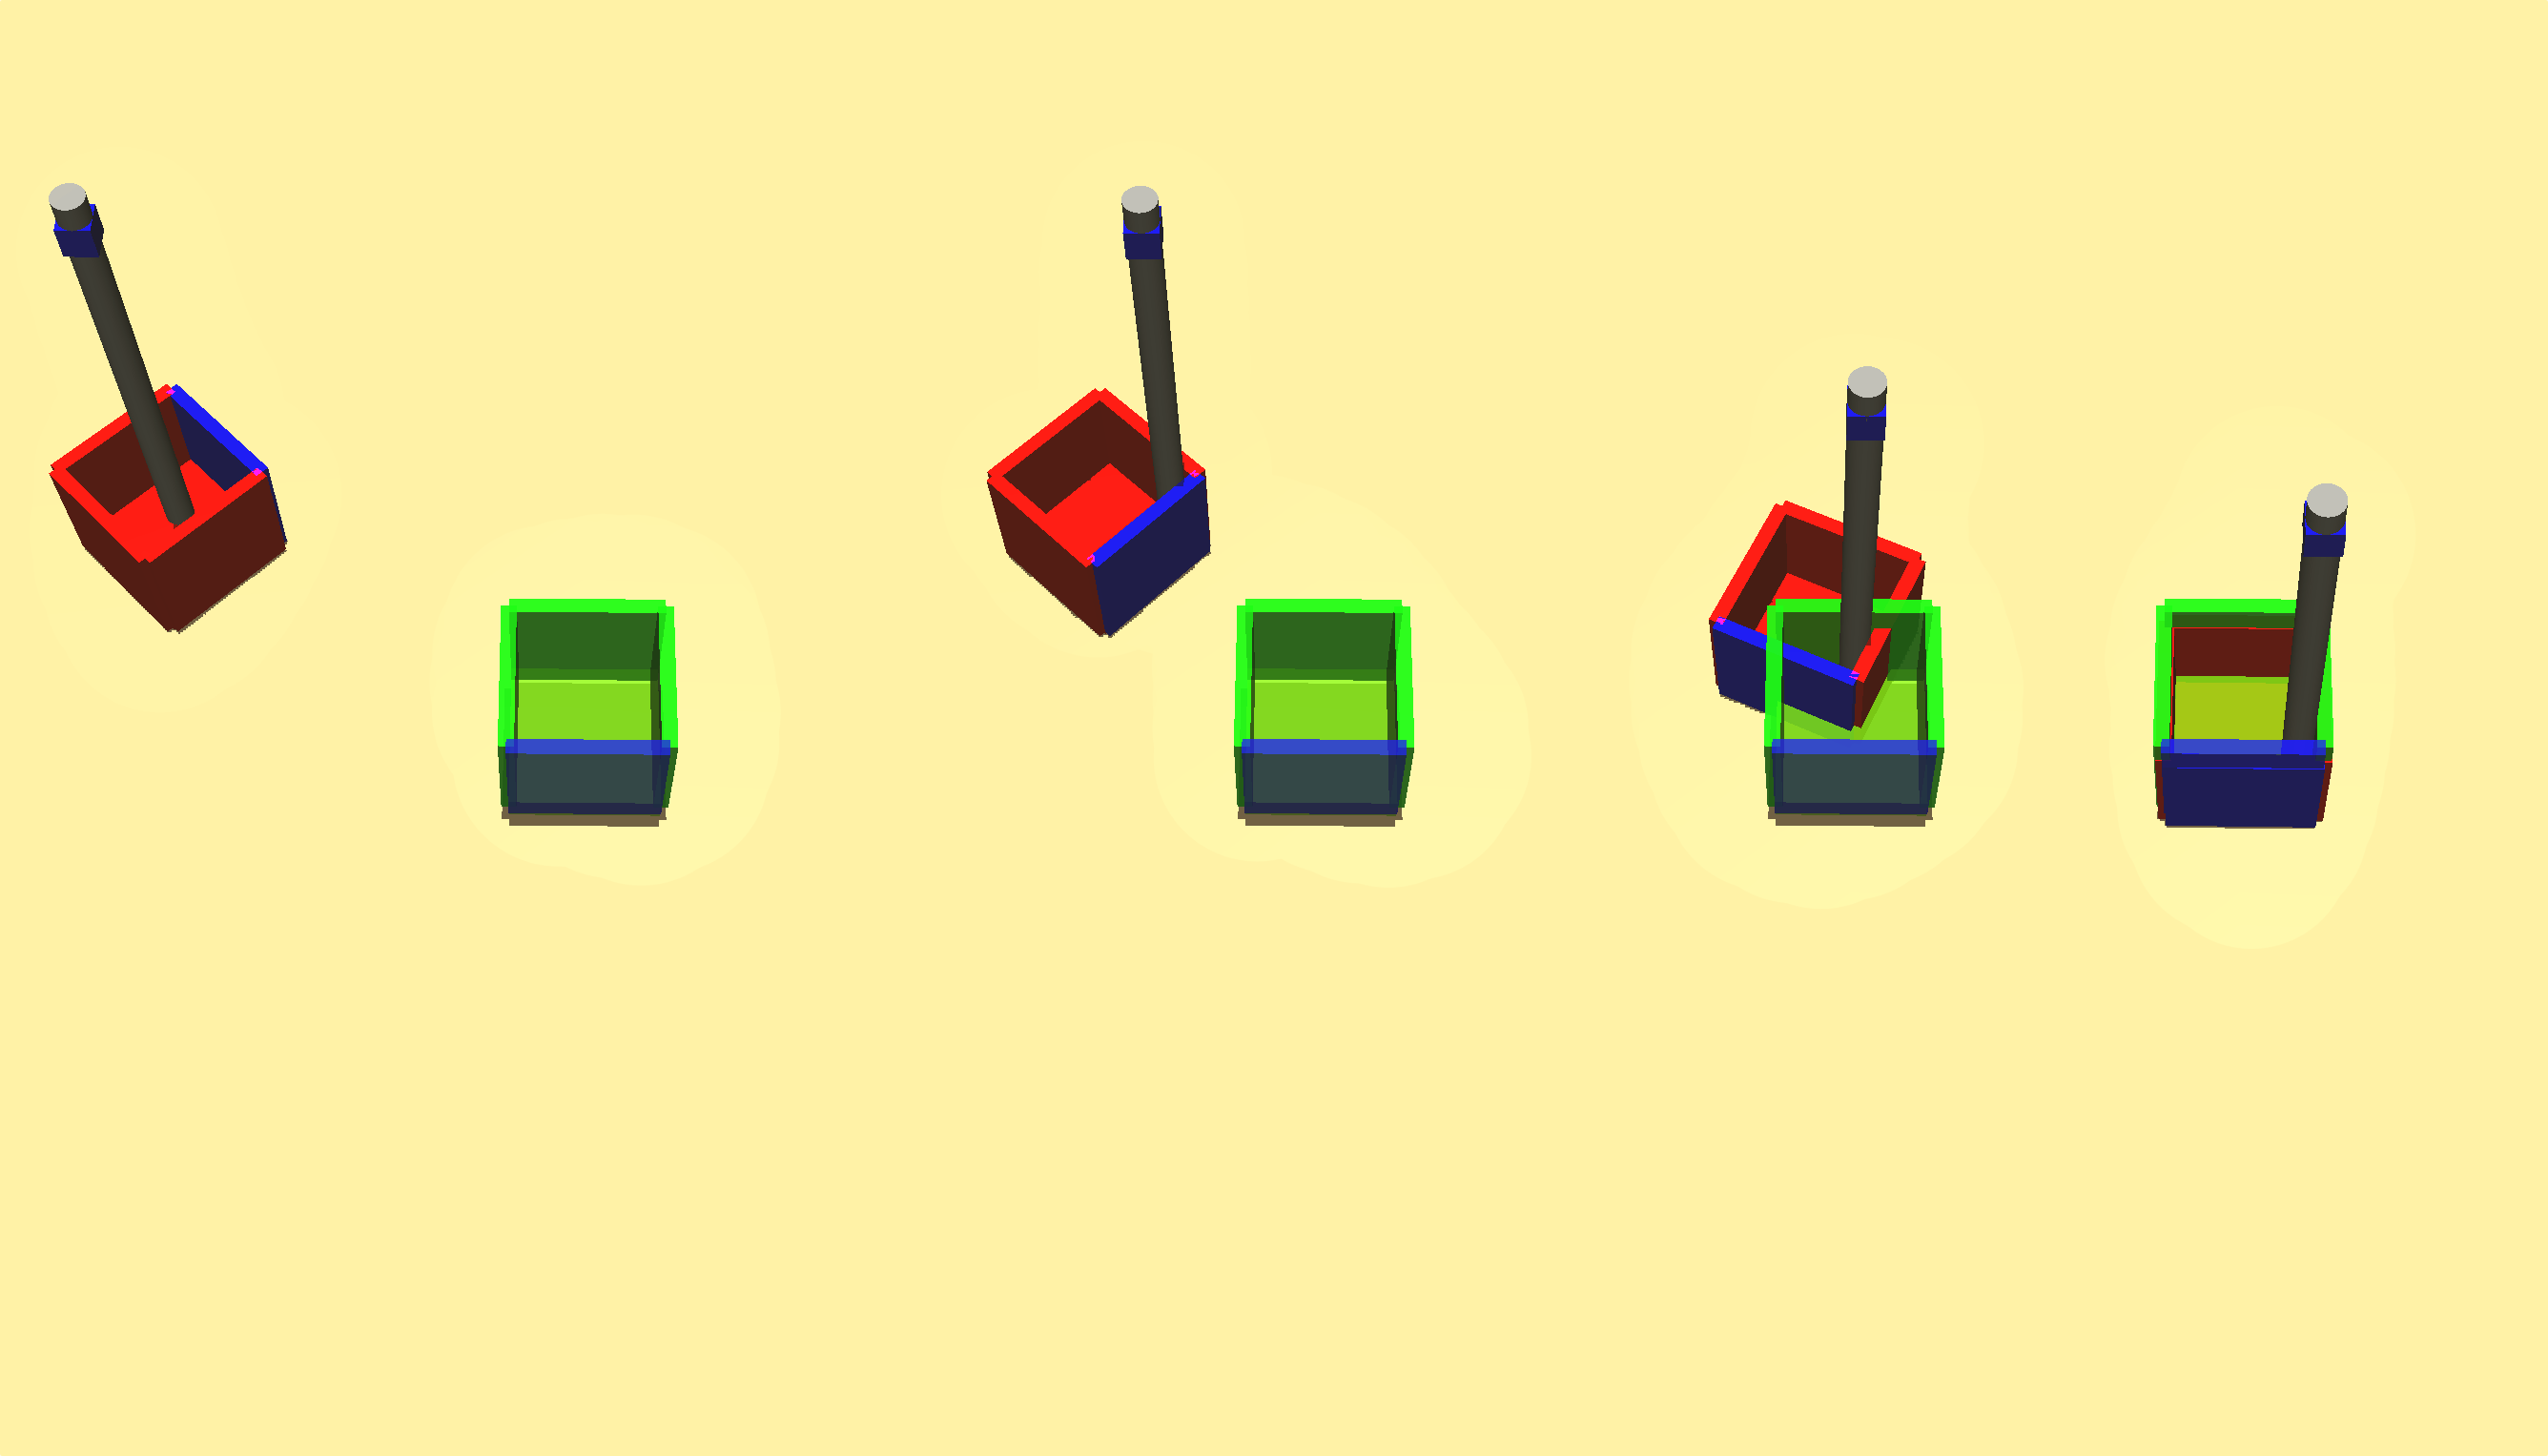
\includegraphics[height=3cm]{media/2dboxpushing.png}
    \vspace{.1cm}\\
    Box Pushing is a challenging benchmark problem for motion primitive reinforcement learning.
\end{frame}

\begin{frame}{Box Pushing}

\begin{columns}[t]
    \begin{column}{0.4\textwidth}
        \vspace{1cm}
        \begin{itemize}
            \item Goal: Use a finger to push a box to a target pose
                \begin{itemize}
                    \item Random start pose
                    \item Fixed target pose
                \end{itemize}
            \item Action space: 2D finger positions
            \item Observation:
                \begin{itemize}
                    \item Finger position
                    \item Box quaternion + noisy position
                \end{itemize}
            \item Success
                \begin{itemize}
                \item $\text{err}_{position} \leq 5 \text{cm}$
                \item $\text{err}_{rotation} \leq 0.5 \text{rad}$
                \item $\max_t(v_t) < v_\text{max}$
                \end{itemize}
        \end{itemize}
            \vspace{1em}
    \end{column}
    \begin{column}{0.5\textwidth}
        \vspace{.5cm}
        \[
        \begin{aligned}
            \text{Reward} &:= \textcolor{kit-blue100}{\text{Final Euclidean Distance}} \\
             &+  \textcolor{kit-blue100}{\text{Final Rotational Distance}} \\
             &+  \textcolor{kit-blue100}{\mathds{1} \left\{\text{success}\right\} } \\
             &-  \textcolor{kit-green100}{\max_t\  \text{step}(v_t)} \\
             &-  \textcolor{kit-lila100}{\sum_t \left\Vert x_t - x_t^\text{clipped} \right\Vert }\\
             \\
    step(v) := & 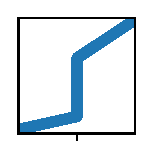
\includegraphics[scale=.4]{media/step.pdf} \\
        \end{aligned}
    \]

    \end{column}
\end{columns}
\center
    Our reward includes \textcolor{kit-blue100}{sparse}, \textcolor{kit-green100}{non-markovian} and \textcolor{kit-lila100}{dense} components.
\end{frame}

\subsection{Making it work in Simulation}
\begin{frame}{Box Pushing --- In Simulation}

\begin{columns}[t]
    \begin{column}{0.4\textwidth}
        \vspace{1cm}
        \begin{itemize}
            \item Box Pushing is \textbf{hard}.
            \begin{itemize}
                \item It took long to get $60-80$\% success in sim 
                \item 127 Sweeps so far, 2628 policies trained
                \item $\approx 25-50\text{M}$ sim steps per policy 
                \item $\approx 60-120\text{K}$ 4s trajectories
            \end{itemize}
            \item So many parameters:
            \begin{itemize}
                \item Reward coefficients
                \item Maximum Speed $v_{\max}$
                \item Amount of randomization
                \item Episode Length
                \item MP Parameters
                \item TRPL Hyperparameters
            \end{itemize}
        \end{itemize}
    \end{column}
    \begin{column}{0.5\textwidth}
        \vspace{.2cm} \\
        \center 
        \includegraphics[width=.5\linewidth]{../fancy_gym/sweeps.pdf} \\

    \end{column}
\end{columns}
\end{frame}

\subsection{Making it work on the real Robot}

\begin{frame}{Box Pushing --- Making it work on the real Robot}
\begin{columns}
    \begin{column}{0.5\textwidth}
        \begin{itemize}
                \item No controller tracks perfectly
                \item The agent will \textbf{adapt} to the simulated controller under- or overshooting.
                \item Also the real robot trajectory has artifacts because of the 7DoF kinematics
                \item \textbf{Tuning for the real robot is crucial!}
        \end{itemize}
    \end{column}
    \begin{column}{0.5\textwidth}
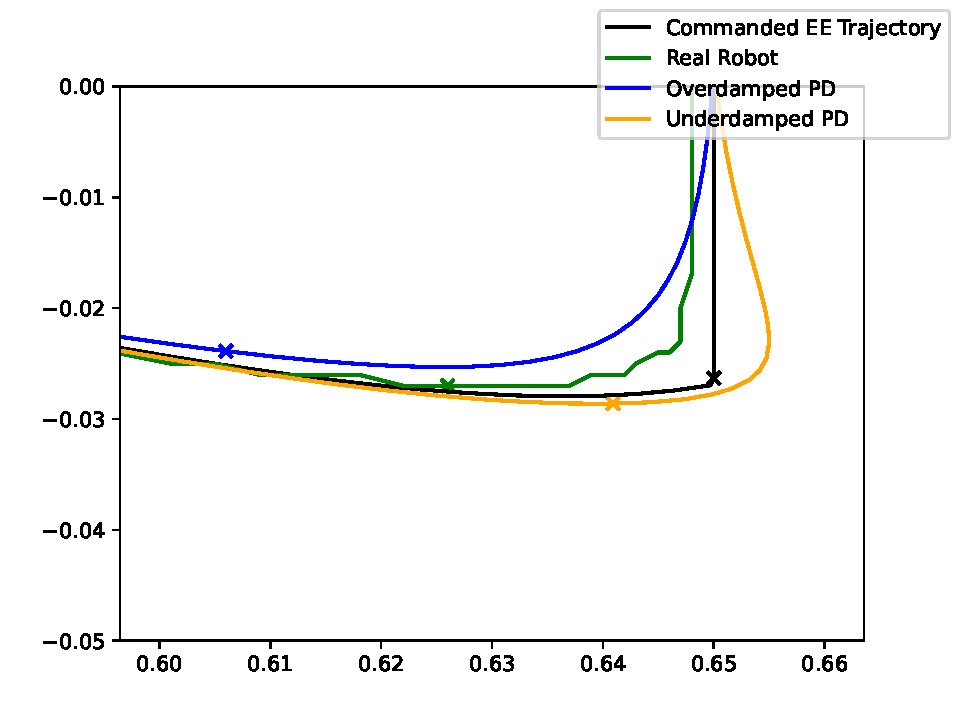
\includegraphics[width=\linewidth]{media/traj_error.pdf}
    \end{column}
\end{columns}

\end{frame}
\begin{frame}{Box Pushing --- Making it work on the real Robot}
\begin{columns}
    \begin{column}{0.5\textwidth}
        \begin{itemize}
                \item Our approach:
                    \begin{itemize}
                            \item Record real-robot executions
                            \item Optimize simulation PD parameters using bayesian optimization
                            \item Choose a lower/higher P-gain 
                            \item Sample $Kp \sim \text{U}(Kp^-, Kp^+)$ during training
                    \end{itemize}

                    \[
                        \min_{kp, kd, mass} \sum_t \left\Vert x_t^\text{real} - x_t^\text{sim}(kp, kd, mass) \right\Vert
                    \]
        \end{itemize}
    \end{column}

    \begin{column}{0.5\textwidth}
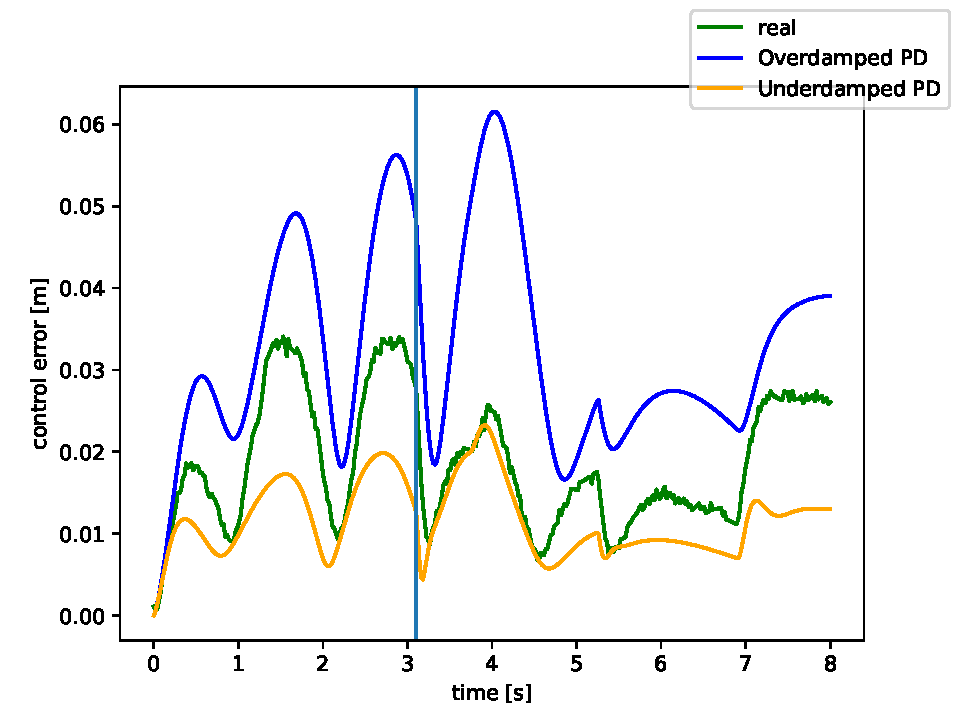
\includegraphics[width=\linewidth]{media/ctrl_error.pdf}\\
    \end{column}
\end{columns}

\end{frame}

\section{Rollout Architecture}
\begin{frame}{Rollout Architecture}
    \begin{columns}
    \begin{column}{0.45\textwidth}
    \vspace{1cm}
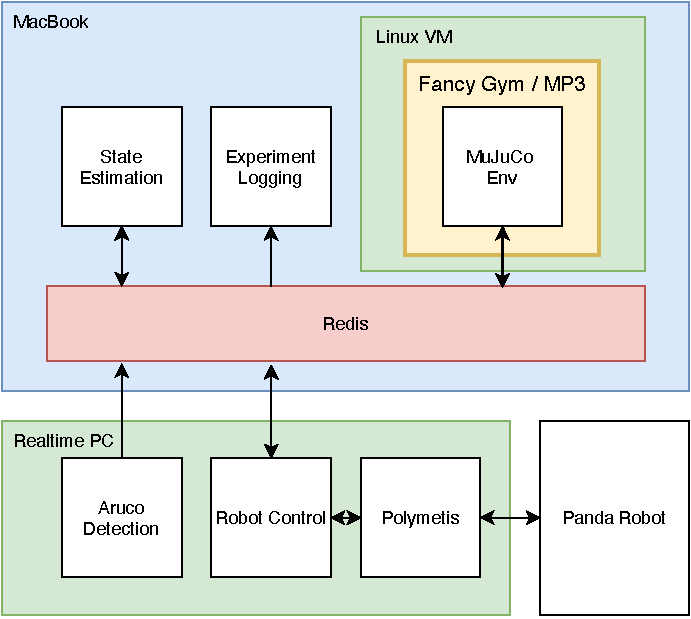
\includegraphics[width=\linewidth]{media/Architecture2.pdf}

    \end{column}
    \begin{column}{0.35\textwidth}
    \vspace{1cm}
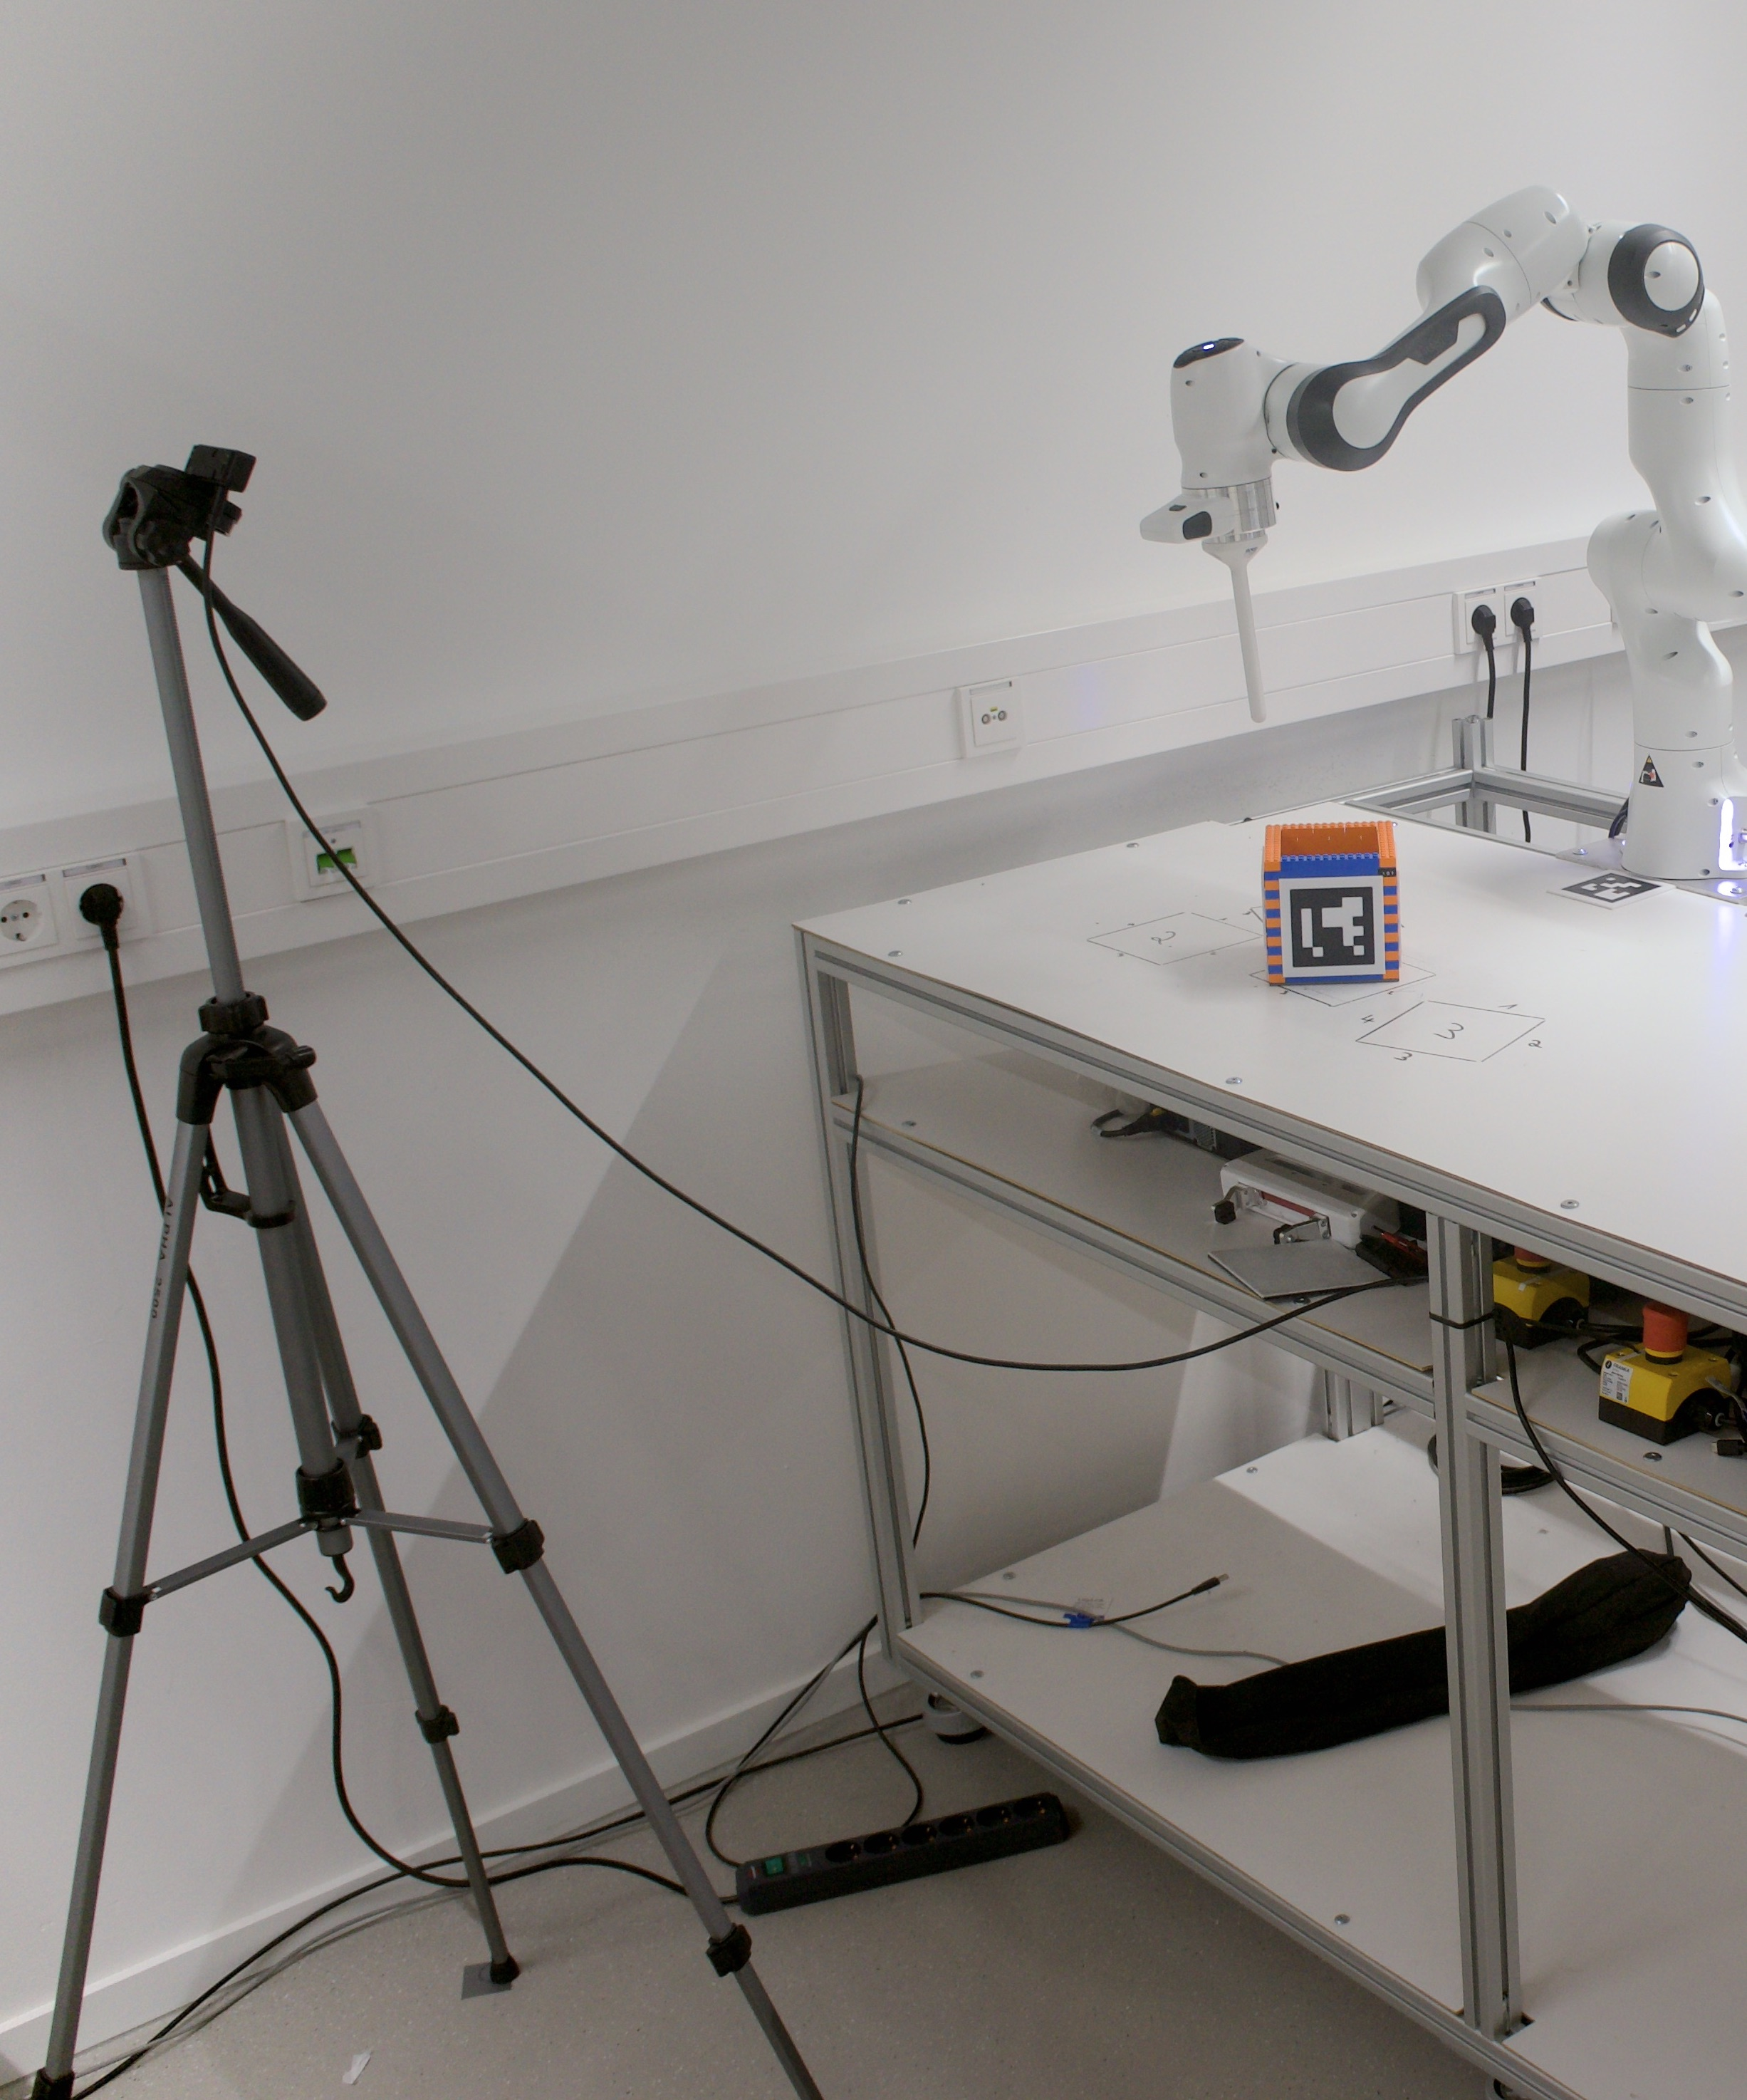
\includegraphics[width=\linewidth]{media/labsetup2.jpg}

    \end{column}
    \end{columns}

\end{frame}

\begin{frame}{Real World Evaluation}
    \center
    Small Demo
\end{frame}

\section{Results}
\begin{frame}{Results}
\center
    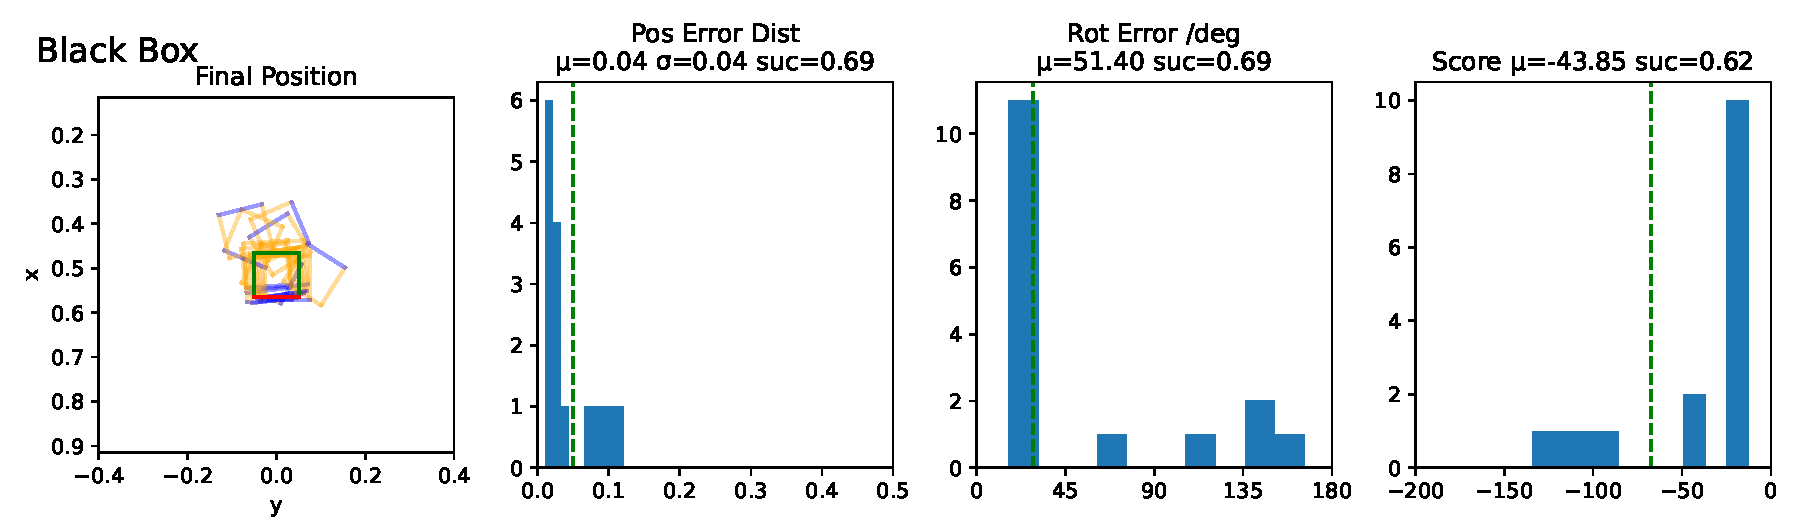
\includegraphics[width=.7\linewidth]{media/blackbox_presentation.pdf}\\
    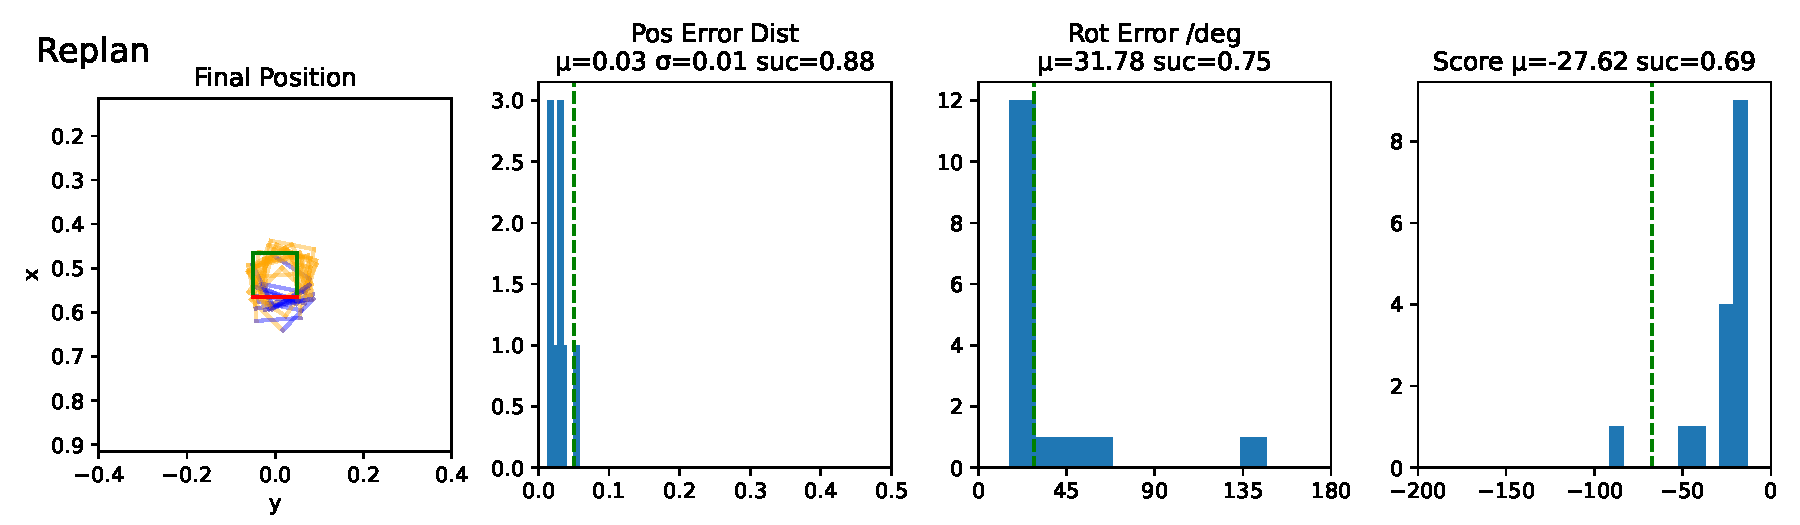
\includegraphics[width=.7\linewidth]{media/replan_presentation.pdf}
\end{frame}

\section{Next Steps}
\begin{frame}{Next Steps}

    \begin{itemize}
        \item Push to 90\% real-life success 
        \begin{itemize}
                \item I think its 50/50 between sim2real and general model performance
        \end{itemize}
        \item Move inference away from my laptop 
        \item Comparison with step-based methods
        \item Proper ablation studies
    \end{itemize}
\end{frame}


\appendix
\beginbackup{}
\begin{frame}{Box Pushing --- Clipping }
    \begin{columns}
    \begin{column}{0.4\textwidth}
        \vspace{.1cm}
        \[ \text{Reward}_{\text{clipping}} := \sum_t \left\Vert x_t - x_t^\text{clipped} \right\Vert \]
        \begin{itemize}
            \item Idea: Penalize the agent for \textbf{leaving the working area}
            \item Outside of the working area, the policy is \textbf{ineffective}
            \item Without the reward, the agent\dots 
            \begin{itemize}
                    \item spent 80\% of its time outside the working area
                    \item never learned to correct this
                    \item exceeded the maximum speed $v_\text{max}$
            \end{itemize}
        \end{itemize}
    \end{column}
    \begin{column}{0.6\textwidth}
        \vspace{.1cm}
    \center
    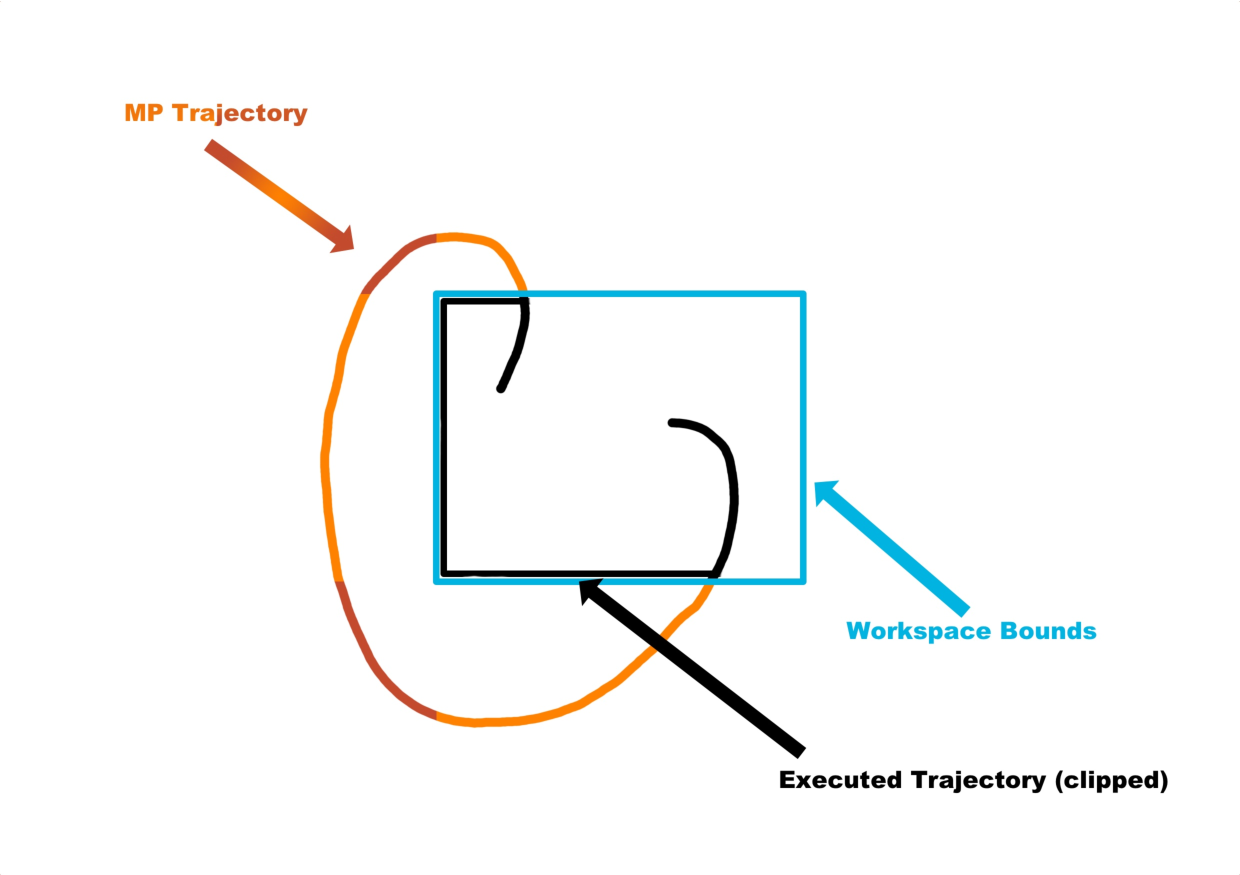
\includegraphics[width=\linewidth]{media/workspace_clipping.pdf}

    \end{column}
    \end{columns}
\end{frame}

\begin{frame}{Box Pushing --- Clipping}
      
\begin{columns}       
     \begin{column}{0.4\textwidth}
        \vspace{1cm}
        \begin{itemize}
                \item Clipping penality has a big effect on performance
                \item Every MP Env should have one
        \end{itemize}
    \end{column}
    \begin{column}{0.6\textwidth}
        \vspace{.2cm} \\
        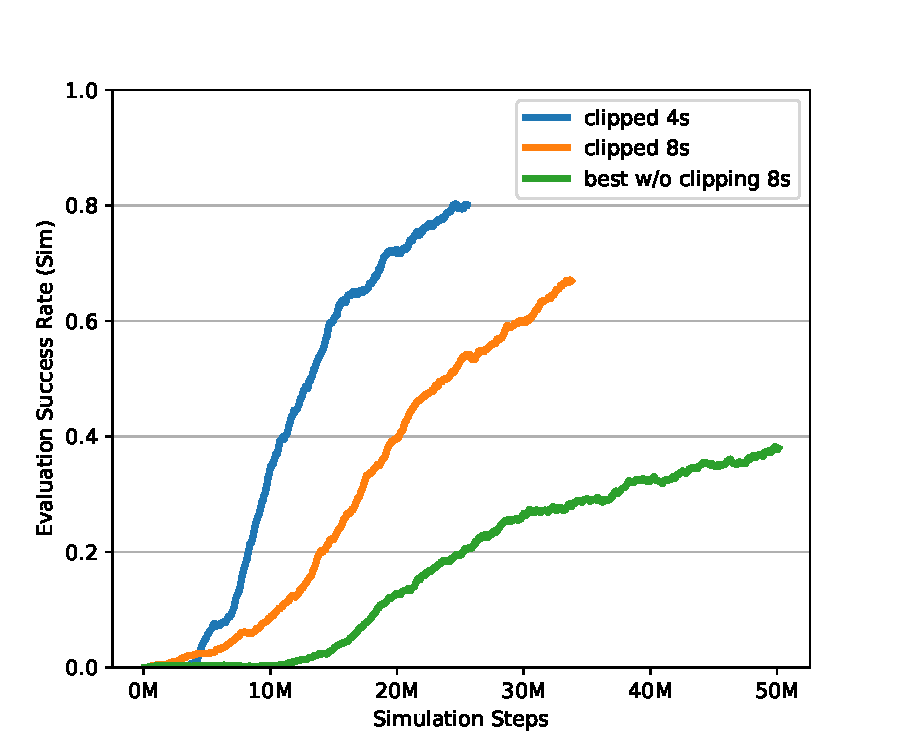
\includegraphics[width=\linewidth]{media/clipping_reward.pdf}

    \end{column}
\end{columns}       
\end{frame}


\backupend{}

\end{document}
